% Chapter Template


\chapter{Experiments} % Main chapter title

\label{experiments} % Change X to a consecutive number; for referencing this chapter elsewhere, use \ref{ChapterX}
Several experiments were conducted on the human parts and keypoint detection modules.
In fact, the resulting network architecture from the human parts module was applied later to the background extraction module.
All in all, eight network architecture variants differentiating in commonly discussed parameters presented in \autoref{theory}
were investigated.
For the keypoint detection module, tests with and without \code{Dense} layers were conducted.
On the human parts detection module, the three state-of-the-art optimizers \textit{Adam, Nadam,} and \textit{SGD} were tested and little
modifications to the \textit{SGD} optimizer were experimented with.
To overcome class invariance, three different loss functions were examined of which one as developed in the scope of this research work.
In the subsequent sections the experimental setup, results, and constructive thoughts behind the studies will be explained.
%----------------------------------------------------------------------------------------
%	SECTION 1
%----------------------------------------------------------------------------------------

% with custom loss function and Adam optimizer_kps


%\section{Different Net Architectures}
\section{Ablation Study}



%-----------------------------------
%	SUBSECTION 1
%-----------------------------------

\begin{table}[]
\begin{footnotesize}
    \caption[Ablation Human Parts Module]{Ablation Human Parts Module: Network Architecture Comparison} \label{table:ablation}
\begin{tabular}{Nlllll}
\hline
\multicolumn{1}{|c}{} &
  \textbf{Name} &
  \textbf{\begin{tabular}[c]{@{}l@{}}Parameter \\ Amount\end{tabular}} &
  \textbf{\begin{tabular}[c]{@{}l@{}}Trainable \\ Parameters\end{tabular}} &
  \textbf{Layers} &
  \textbf{\begin{tabular}[c]{@{}l@{}}Training \\ Time/Epoch\end{tabular}} \\ \hline
\label{HRNet:traditional} & \begin{tabular}[c]{@{}l@{}}HRNet \\ \textit{- traditional}\end{tabular}          & 5,595,221 & 5,589,237 & 171 & 84.76s \\ \hline
\label{HRNet:filter} & \begin{tabular}[c]{@{}l@{}}HRNet \\ \textit{- adjusted filter}\end{tabular}      & 4,936,997 & 4,933,029 & 171 & 66.23s \\ \hline
\label{HRNet:3s} & \begin{tabular}[c]{@{}l@{}}HRNet \\ \textit{- 3 stages}\end{tabular}             & 848,409   & 846,441   & 100 & 82.33s \\ \hline
\label{HRNet:stride} & \begin{tabular}[c]{@{}l@{}}HRNet \\ \textit{- stride-down-up}\end{tabular}       & 4,953,269 & 4,949,157 & 177 & 63.21s \\ \hline
\label{HRNet:stride-i} & \begin{tabular}[c]{@{}l@{}}HRNet \\ \textit{- stride-down-up-input}\end{tabular} & 4,185,605 & 4,181,493 & 177 & 80.57s \\ \hline
\label{HRNet:add-i} & \begin{tabular}[c]{@{}l@{}}HRNet \\ \textit{- add-input}\end{tabular}            & 4,185,605 & 4,181,493 & 177 & 80.57s \\ \hline
\label{HRNet:add-dwconv} & \begin{tabular}[c]{@{}l@{}}HRNet \\ \textit{- add-depthwise-conv}\end{tabular} & 3,182,342 & 3,177,654 & 156 & 83.10s \\ \hline
\label{UNet} & UNet                                                                    & 656,389   & 654,261   & 88  & 85.37s \\ \hline
\label{HRNet:v3} & \begin{tabular}[c]{@{}l@{}}HRNet \\ \textit{- v3}\end{tabular}                   & 3,008,562 & 3,003,930 & 156 & 85.43s \\ \hline
\end{tabular}
    \end{footnotesize}
\end{table}
\setcounter{rowcntr}{0}


\subsection{Body Parts Detection Module }
\label{RBP}

In~\ref{fig:ablation-accuracy} the in this research work developed network architectures are outlined.
These range from 88 until 177 layers and are
all fully convolutional networks.
For the HRNet \textit{(traditional)}~\ref{HRNet:traditional} the HRNetV2 presented in~\cite{HRNetv2} was slightly deviated
by replacing the \code{Pooling}
layers with \code{strided-down} and \code{transposed convolutional} layers.
The amount of levels and sizes of the feature maps correspond to~\ref{fig:custom_hrnet}.
As in HRNetV2 4 stages are used with a filter size of 64 for each stage.
One additional level per stage starting with just the highest level $\mathcal{N}_L$
and the concatenations of the levels from stage 2 ongoing are demonstrated with HRNetV2.\\
For the HRNet \textit{(filters)}~\ref{HRNet:filter}, the filters are adjusted in a way, so that higher levels use fewer filters then lower levels.
Additionally, the filter amount of the \code{convolutional} layers is decreased in the level blocks, starting from the highest filter
amount, and reducing until 36.
All levels are \code{concatenated} with a filter size of 36.\\
Subsequent architectures all make use of the adjusted filter amount.\\
For the HRNet \textit{(3 stages)}~\ref{HRNet:3s}, only the three first stages from~\ref{HRNet:filter} are used and
$\mathcal{N}_{XS}$ is omitted.\\
In HRNet \textit{(stide-down-up)}~\ref{HRNet:stride}, the Input from 240x320x3 is strided down to 120x160x36 and this layer is used as \code{Input} layer
and highest level block $\mathcal{N}_L$. Lower layers scale relatively to $\mathcal{N}_L$.
The HRNet \textit{stride-down-up-input}~\ref{HRNet:stride-i} uses the initially strided down \code{Input} layer as input for
every stage instead of the concatenated results of lower levels.\\
As presented in the \textit{MobileNet} paper~\cite{mobilenet} in~\ref{HRNet:add-dwconv} \code{depth-wise convolution} is experimented with
and the \code{Concatenation} layers are replayed after each stage with \code{Add} layers.\\
In the UNet~\ref{UNet} all levels are used and combined via \code{concatenation} according to the traditional UNet~\cite{unet}.\\
Finally, the resulting high-to-low resolution network HRNet \textit{(v3)}~\ref{HRNet:v3} is presented, where
the first stages are fused and only concatenate the last stage is concatenated. Furthermore, some adjustments to the layer amount
in the levels and stages where applied as presented in~\autoref{method}.
\\\mbox{}\\
The HRNet stride-down-up~\ref{HRNet:stride} seems to train the fastest, when looking at~\ref{fig:ablation-correct-px} the
4.705kth step, it is only at three days and 13h closely followed by the traditional HRNet with the adjusted filters~\ref{HRNet:add-dwconv}
which is at 3 days and 13h. All other trainings took more than four days at that time.
However, one has to keep in mind that both trainings where conducted at the same dates, and the other dates differ.
So the server could have had other workloads, nevertheless, the trainings were the only ones running on the server most
of the time. This occasion as well is reflected in the training time of one epoch.
There as well both the HRNet \textit{stride-down-up} and HRNet \textit{adjusted-filter} only took about ~63, ~66 seconds,
where all the others took more then 80 seconds.
However, one would have expected the U-Net or HRNet \textit{3 stages} to be the fastest since they have the smallest
amount of layers and trainable parameters.
Further, the HRNet \textit{stride-down-up-input} contains less trainable parameters then \textit{stride-down-up}, so
one would have expected a faster training process there.
This verifies that the measurements are dependent on various circumstances.
Indeed, to improve comparability, only the third epoch was measured to omit starting warm up phases.


\subsubsection{Comparison of Network Architectures}
%
The U-Net~\ref{UNet} has the smallest amount of layers with 88 and 654,261 trainable parameters.
The HRNet \textit{stride-down-up}~\ref{HRNet:stride} composes most trainable parameters with 4,949,157 and 177 layers, since the Input
layer is first strided down and at the end transposed up again.
On the other hand, due to the reduced feature map sizes, this reduces the computation effort as well.
All comparison figures show very similar curves.
Since the experiments could only be performed one complete training each, the results must be viewed circumspectly.
All figures~\ref{fig:ablation-accuracy, fig:ablation-correct-px, fig:correct-pixel-ratio} show very steep curves until
the 500th episode and start to flatten then.\\
When looking at~\ref{fig:train-img-0} and~\ref{fig:train-img-20} this steep initial increase is visually reflected.
Even if, after the first episode the circumferences of the body shapes are predicted vaguely, after the 20th episode the
networks have already learned to predict the locations of body parts relatively close to the real ones.
Of course, there has to be regarded, that the different predictions were made on different poses, which might differ in
their complexity.
Nevertheless, the UNet~\ref{UNet} and the HRNetV3~\ref{fig:hp_accuracy_hrnet_v3} seem to accomplish superior performance.
After the first episode, the body shape is already estimated precisely close to the input image.
HRNetV3 even shows correct class estimations for different body parts such as the torso, head, arms, and legs already.
In the 20th episode then the labels seem to be estimated very close to the true labels.

\begin{figure}[H]
    \centering
    \includegraphics[width=\textwidth, height=\textheight, keepaspectratio]{Figures/ablation_study_hp_accuracy.png}
    \decoRule
    \caption[Ablation Human Parts Module: Accuracy]{Ablation Human Parts Module: Accuracy Comparison}
    \label{fig:ablation-accuracy}
\end{figure}

The accuracy graph shows that the HRNet \textit{(traditional)} and HRNetV3 get the best results from epoch 500 onwards.
At step 55.55k they reach 99 percent.
However, the HRNet \textit{(stride-down-up)} has a lower curve until the 4.3k$^{th}$ epoch, it then makes a jump in accuracy
and at the end reaches 99 percent as well.
Interestingly the U-Net with the by far fewest parameters and layers does receive very good results as well making almost
99 percent in accuracy at the end.
The HRNet with only three stages shows the lowest curve and reaches only 98.87 percent points on accuracy at the end.

\begin{figure}[H]
    \centering
    \includegraphics[width=\textwidth, height=\textheight, keepaspectratio]{Figures/ablation_study_hp_correct_pixel.png}
    \decoRule
    \caption[Ablation Human Parts Module: Correct Pixel]{Ablation Human Parts Module: Correct Pixel}
    \label{fig:ablation-correct-px}
\end{figure}

The correct pixel graph~\ref{fig:ablation-correct-px} measures how many pixels of the 240x320 image where predicted correctly
in one batch. The maximum which could be reached is $240\times320\times3=\numprint{230400}$.
Since the single epochs vary a lot, it makes more sense to look at the smoothed results.
The curves again are very close to each other, with the best results coming from the HRNetV3 with $\numprint{219670}$ and
the HRNet \textit{traditional} with $\numprint{219640}$.
The lowest curve again shows the HRNet \textit{3 stages}.

\begin{figure}[H]
    \centering
    \includegraphics[width=\textwidth, height=\textheight, keepaspectratio]{Figures/ablation_study_hp_bp_pixel_ratio.png}
    \decoRule
    \caption[Ablation Human Parts Module: Correctness Ratio]{Ablation Human Parts Module: Correct Pixel Ratio}
    \label{fig:correct-pixel-ratio}
\end{figure}

For~\ref{fig:correct-pixel-ratio} the amount of body part pixels was summed up and divided by the amount of correctly
predicted pixels for one training batch.
This figure as well displays high variances for the different epochs, which is why it is important to take the smoothed
values into account. Similar courses are received as already inspected in~\ref{fig:ablation-correct-px}.
The HRNet \textit{(traditional)} and HRNetV3 take the lead wih the \textit{(traditional)} one being slightly above the HRNetV3
with 0.05 percent points. With 31.44 percent the HRNet \textit{(traditional)} shows the best results, whereas HRNet
\textit{(3 blocks)} performs worst with 30.38 percent at step 4.93k.

\begin{figure}[H]
    \centering
    \includegraphics[width=\textwidth, height=\textheight, keepaspectratio]{Figures/ablation_study_train_imgs_0.png}
    \decoRule
    \caption[Ablation Human Parts Module: 1st Episode Predictions]{Predicted images of network architectures after first
    episode}
    \label{fig:train-img-0}
\end{figure}
\begin{figure}[H]
    \centering
    \includegraphics[width=\textwidth, height=\textheight, keepaspectratio]{Figures/ablation_study_train_imgs_20.png}
    \decoRule
    \caption[Ablation Human Parts Module: 20th Episode Predictions]{Predicted images of network architectures after 20th
    episode}
    \label{fig:train-img-20}
\end{figure}

\paragraph{Summary}\mbox{}\\
In summary, the here presented experiments show that the in this thesis constructed HRNetV3 performs best, and the HRNet with only three stages performs
worst.
Interesting here would be to investigate the different variations in the level of feature map sizes.
For instance what would happen if the level $\mathcal{N}_{XS}$ was maintained as smallest level and the level
$\mathcal{N}_M$ was strided down slightly more?
Insightful as well is the performance of the UNet, which has less than half of trainable parameters and layers compared to
the HRNet \textit{traditional} or HRNetV3, but does not perform much worse.
Additionally, further tweaks and studies in these network architectures applied to the different modules would be
greatly enlightening for further studies.


%-----------------------------------
%	SUBSECTION 2
%-----------------------------------
\subsection{Joint Detection Module }

\begin{table}[H]

%\begin{footnotesize}
    \caption[Ablation Keypoint Module]{Ablation Keypoint Detection Module: Network Architecture Comparison} \label{table:ablation-kp}
\begin{tabular}{|Nlllll|}
    \hline
\multicolumn{1}{|c}{} &
  \textbf{Name} &
  \textbf{\begin{tabular}[c]{@{}l@{}}Parameter \\ Amount\end{tabular}} &
  \textbf{\begin{tabular}[c]{@{}l@{}}Trainable \\ Parameters\end{tabular}} &
  \textbf{Layers} &
  \textbf{\begin{tabular}[c]{@{}l@{}}Training \\ Time/Epoch\end{tabular}} \\ \hline
\label{kps-dense-blockl} & \begin{tabular}[c]{@{}l@{}}KPS-Dense \\ \textit{- block\_L}\end{tabular}          & 221,748,579 & 218,735,769 & 51 & 68.75s \\ \hline
\label{kps-dense} & \begin{tabular}[c]{@{}l@{}}KPS-Dense\end{tabular}      & 23,097,980 & 20,086,328 & 13 & 67.05s \\ \hline
\label{kps-hrnet} & \begin{tabular}[c]{@{}l@{}}KPS-FCN\end{tabular}             & 4,119,529 & 1,109,991 & 41 & 63.78s \\ \hline
\end{tabular}
    %\end{footnotesize}
\end{table}
\setcounter{rowcntr}{0}

\subsubsection{Network Architectures}
The subsequent presented experiments are based on
three created variations of keypoint detection network architectures of which two\ref{kps-dense, kps-dense-blockl}
utilize Dense layers to estimate the keypoint locations and KPS-FCN~\ref{kps-hrnet} implements the third stage of our
build HRNetV3.
KPS-Dense~\ref{kps-dense-blockl}, additionally to the Dense stage, utilizes the third stage of the HRNetV3.\\
The Dense stage first uses max pooling to reduce the feature map size from 240x230x9 to 120x160x1, 58x78x32, and then 28x38x64.
The resulting \code{Pooling} layer is flattened and followed by two Dense layers, which are combined with Dropout and
batch normalization.
The layers include 1024 and 512 units.
The first Dense layer is connected to a Softmax activation function,
the second to a linear activation function. The model estimates 38 x,y coordinates for the human joint locations.
The network's loss function calculates the distance from the predicted keypoint locations to the true locations and optimizes
the network's via mean-squared-error.
In fact, the KPS-FCN~\ref{kps-hrnet} only uses convolutional layers.
The true labels calculate Gaussians with a radius size of three for the locations of the keypoints.
The keypoint classes are combined for equal body locations such has legs and arms, resulting in 11 joint classes.
This network predicts 11 different labels for the classes, and is further optimized with mean-squared-error.
%
All networks are trained with an Adam optimizer with a learning rate of 0.001 and run for 5556 epochs.
%
\begin{figure}[H]
    \centering
    \includegraphics[width=\textwidth, height=\textheight, keepaspectratio]{Figures/ablation_study_kps_imgs.png}
    \decoRule
    \caption[Ablation Keypoints Detection Module: Predicted Training Images]{Predicted images of keypoint detection networks
    after first, 20th and last episode}
    \label{fig:kps-train-imgs}
\end{figure}
%
Both figures~\ref{fig:kps-map-loss},~\ref{fig:kps-loss} show similar curves.
Until the 500th episode they decrease steeply and then they start to flatten.
KPS-Dense~\ref{kps-dense} has the fewest layers with 13, however KPS-FCN~\ref{kps-hrnet} contains only 1,109,991
trainable parameters, the dense networks train \~20/ \~218 times more parameters.
The networks only differ slightly in their training epoch time and are all between 63 and 69 seconds.\\
The main difference though is visible in the predicted training images in~\ref{fig:kps-train-imgs}.
The keypoint detection modules seem not to learn the locations of the body parts, but that the probability of the location
of a keypoint being at the center of the image is much more likely than outer locations.
Very interesting about the KPS-FCN is that this network first learns the locations of the feet, and then slowly goes
upward per epoch learning the other keypoint locations in a continuous way.


\begin{figure}[H]
    \centering
    \includegraphics[width=\textwidth, height=\textheight, keepaspectratio]{Figures/ablation_study_kps_map_loss.png}
    \decoRule
    \caption[Ablation Keypoints Detection Module: Loss FCN]{Ablation Keypoints Detection Module: Loss FCN}
    \label{fig:kps-map-loss}
\end{figure}


\begin{figure}[H]
    \centering
    \includegraphics[width=\textwidth, height=\textheight, keepaspectratio]{Figures/ablation_study_kps_loss.png}
    \decoRule
    \caption[Ablation Keypoints Detection Module: Loss Dense Layers]{Ablation Keypoints Detection Module: Loss Dense Layers}
    \label{fig:kps-loss}
\end{figure}

%-----------------------------------
%	SECTION 2
%-----------------------------------




\subsection{Experiments with Optimizers}
All trainings were conducted with Mini-Batch Gradient Descent and a batch size of three.

\begin{figure}[H]
    \centering
    \includegraphics[width=\textwidth,height=\textheight,keepaspectratio]{img/learning_rate2.png}
    \decoRule
    \caption[Experiments: Learning Rate SGD]{Experiments with Learning Rate SGD.}
    \label{fig:sgd-learning-rate}
\end{figure}
In the here presented experiments \gls{SGD}, \gls{Adam}, and \gls{Nadam} optimization algorithms were tested, all with initial learning rates of $\eta=0.001$.
\gls{SGD} was configured in a way to use Nesterov Momentum with a value of $\gamma=0.9$, \gls{Adam} with epsilon $\epsilon=1e-7$ and AMSGrad.
Nadam used the exponential decay parameters $\beta_1=0.9; \beta_2=0.999$ and epsilon $\epsilon=1e-7$.
Additionally, several tests on the learning rate variations for \gls{SGD} were tested and its influence on the training process was investigated.
One \gls{SGD} configuration is with a constant learning rate $\eta$, one decays with $\eta=0.01$, and one learning rate
decays with $\eta=0.01$, but will reset to the initial learning rate, when no significant learning or changes regarding
the loss value is observed over the last 50 epochs anymore.
Another experiment with \gls{SGD} increases the ascent of decay when a plateau is hit with increasing decay values
$[1e-5, 1e-4, 1e-3, 1e-2]$ as visualized in ~\ref{fig:sgd-learning-rate}.



% https://ruder.io/optimizing-gradient-descent/index.html#nadam

%The goal of gradient descent is to find the minima of the weights, so that the overall error is minimized.
%
%The learning rate is one of the important hyper-parameters, which determines how quickly this minimum can be reached.
%It sets the step size and with it the amount of steps until the model converges.
%So it additionally decides about the training length of the network~\cite{deeplcomputervision}.




%https://mlfromscratch.com/optimizers-explained/#/

\subsubsection{Comparison of Adam, Nadam and SGD}
\begin{figure}[H]
    \centering
    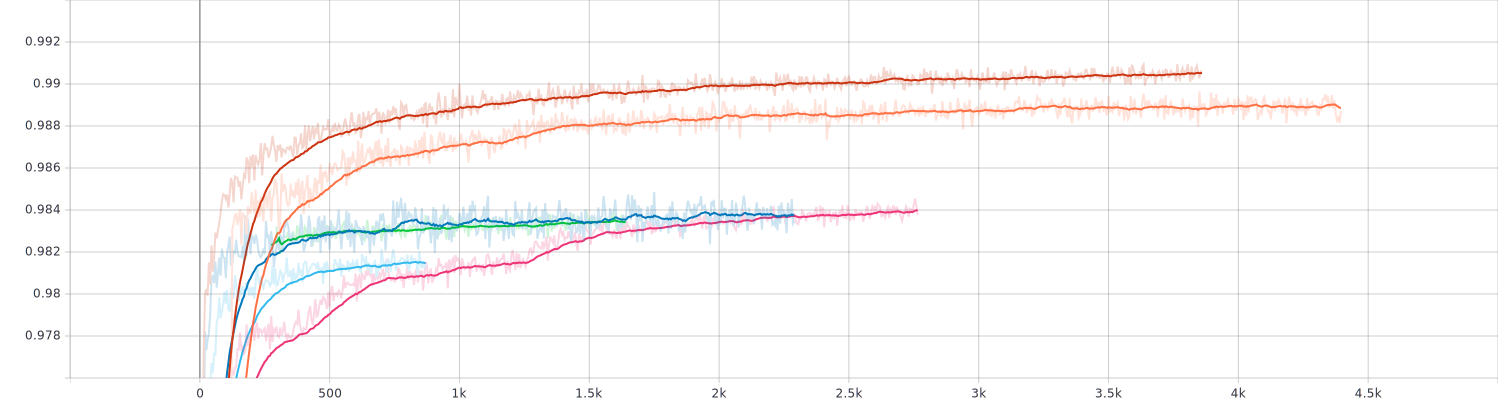
\includegraphics[width=\textwidth,height=\textheight,keepaspectratio]{img/accuracy_all.png}
    \decoRule
    \caption[Experiments: Accuracy]{Accuracy of different optimizer settings}
    \label{fig:accuracy}
\end{figure}

The Figure on accuracy~\ref{fig:accuracy} shows that our network makes huge learning progresses in the first
200 to 300 epochs with an ascent of almost 90 degrees.
However, the graph shows that \gls{SGD} performs worse than \gls{Adam} or \gls{Nadam}, all networks reach a commendable accuracy above
98 percent, whereas \gls{Nadam} even gets over the 99 percent mark.
\gls{Adam} and \gls{Nadam} start to flatten a little bit later than \gls{SGD} about 100 epochs.
Furthermore, their curves flatten more evenly, whereas \gls{SGD}
seems to flatten more abruptly.
Interestingly, the \gls{SGD} optimizer shows jumps in its curve, when the learning rate is resetted when facing a plateau.
There one can observe the typical flattening of \gls{SGD} and then, when a reset took place, the learning process starts again.
This indicates that \gls{SGD} hit a local minimum from which it seems to jump out and re-trigger the adjustment of $\theta$.

%\begin{figure}[H]
%    \centering
%    \includegraphics[width=\textwidth,height=\textheight,keepaspectratio]{img/accuracy_sgd.png}
%    \decoRule
%    \caption[Accuracy SGD]{Accuracy SGD.}
%    \label{fig:sgd-accuracy}
%\end{figure}



%\begin{figure}[H]
%    \centering
%    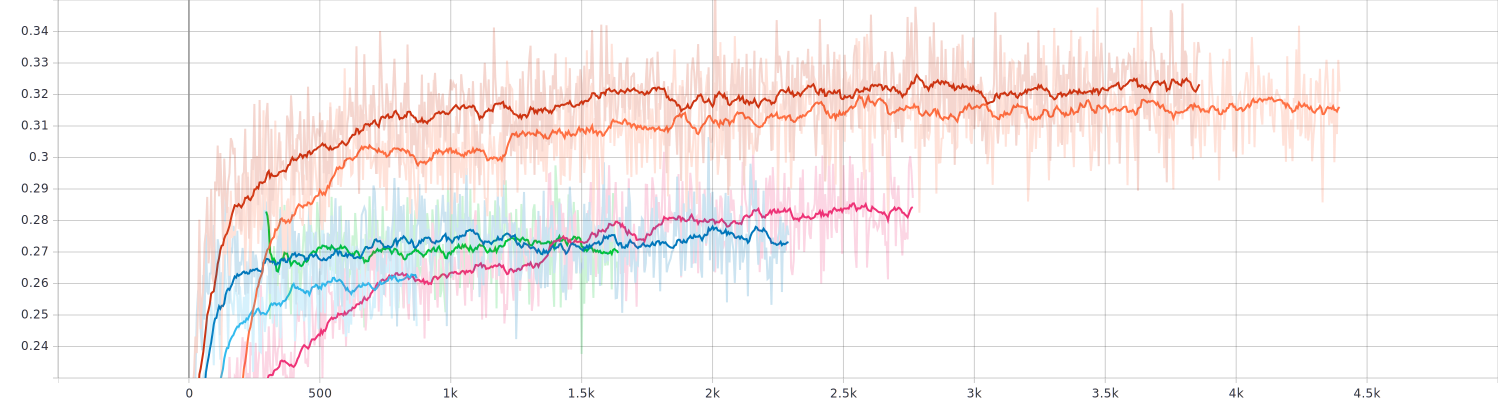
\includegraphics[width=\textwidth,height=\textheight,keepaspectratio]{img/accuracy_body_part_all.png}
%    \decoRule
%    \caption[Correct BPR]{Correct body part pixel relation}
%    \label{fig:acc-bp}
%\end{figure}


\begin{figure}[H]
    \centering
    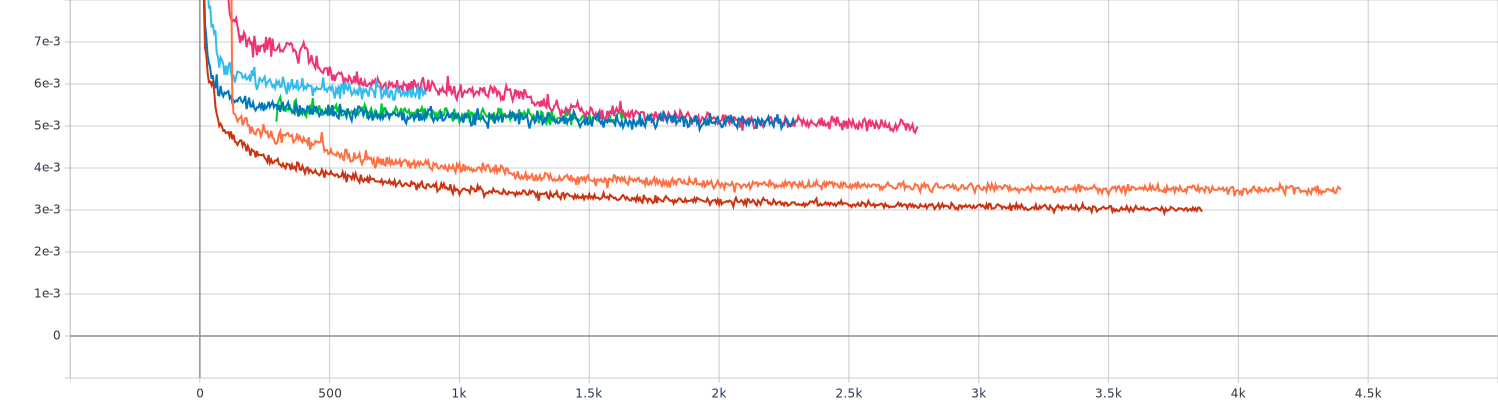
\includegraphics[width=\textwidth,height=\textheight,keepaspectratio]{img/loss_all.png}
    \decoRule
    \caption[Experiments: Loss curves]{Experiments: Loss curves}
    \label{fig:loss}
\end{figure}
Similar process curve trends can be observed in~\ref{fig:loss}, while the curves are mirrored at the x-axis.
This correlation of loss and accuracy trend proves the associate learning process for the different optimizers.


\subsubsection{Conclusions}
The here presented results are reflected by the research from Choi et Al~\cite{empiricaloptimizers}.
They conducted a very interesting research with the thesis that more general optimizers would never underperform
the ones they approximate.
Meaning \gls{RMSProp}, \gls{Adam} and \gls{Nadam} would always perform at least as good if not better than Momentum, Nesterov or \gls{SGD}.
They impose to carefully tune the hyperparameters and not just conclude an optimizer would work better than another one.
This is why in this investigative work very commonly recommended hyperparameters were used and experimented with.
A continuing grid search could help to find an even more efficient way for training and probably even result in better
learned network parameters $\theta$~\cite{gridsearch}.
%\begin{figure}[H]
%    \centering
%    \includegraphics[width=\textwidth,height=\textheight,keepaspectratio]{img/loss_sgd.png}
%    \decoRule
%    \caption[Loss SGD]{Loss SGD.}
%    \label{fig:sgd-loss}
%\end{figure}



%----------------------------------------------------------------------------------------
%	SECTION 3
%----------------------------------------------------------------------------------------


\section{Performance of loss functions}

We trained the Keypoint Detection and Body Part Extraction modules with MSE.

However, with our Body Part Detection Module we initially had problems with class imbalances.
First, we conducted our training with Sparse Categorical Cross Entropy (SCCE)


Nevertheless, our first results~\ref{fig:cross_entropy_pred_img} made us believe that with SCCE our net was not able to
learn the correct labels for the pixels.
Especially the prediction after the 60th epoch shows, that the net mainly has learned to classify all body parts with the
torso class.
We assumed this was the case, because the likeliness of the pixel to be of class torso is higher than, for
example, foot.
Furthermore, however, the accuracy graph shows descent results over 94 percent it started to flatten more and more becoming
almost flat after the 50th epoch already.
\begin{figure}[H]
    \centering
    \includegraphics[width=\textwidth,height=\textheight,keepaspectratio]{Figures/accuracy_cross_entropy.png}
    \decoRule
    \caption[Loss Functions SCCE: Accuracy]{Accuracy for training with Sparse Categorical Cross Enntropy loss function}
    \label{fig:accuracy_cross_entropy}
\end{figure}
\begin{figure}[H]
    \centering
    \includegraphics[width=\textwidth,height=\textheight,keepaspectratio]{Figures/crossentropy_imgs_prediction_last_epoch.png}
    \decoRule
    \caption[Loss Functions SCCE: predictions]{Predicted images for training with Sparse Categorical Cross Entropy loss function}
    \label{fig:cross_entropy_pred_img}
\end{figure}
We then created our own loss function for this class imbalance problem as explained in~\autoref{ciloss}.
Moreover, we reduced the number of classes from 14 to nine accumulating left and right body parts such as foot and arm.
A later experiment shows, on the contrary, that our build network HRNetv3 even learns slightly better than with our own created
loss function CILoss~\ref{fig:ablation-accuracy}.
Even though, this of course could be by chance due to current training circumstances.


\subsection{Custom Developed Loss Function: CILoss}
\label{ciloss}
This loss function confronts the problem of class imbalance, which especially occurs in body part recognition.
The background pixels appear most often, and the different body part classes occur much less often and they even
differ a lot in their relative occurrence.
\\\mbox{}\\
We try to confront this problem with a weighed map $\mu$, which takes the body parts as a graph and calculates
the distances from each body part $b_x$ to all other body parts $b_n$, and store this data inside a table.
This weighed map $\mu$ is applied to the true labels of $y_{true}$ so that wrong predictions further away from the true
class will be punished more. For example if the network predicts hand instead of lower arm, the error will be less as if
the network predicts foot.
\\\mbox{}\\
Additionally, this weight map is evened out with a multiplier to reduce the distances and facilitate
the learning process for the network.
\\\mbox{}\\
As in MSE we calculate the difference $\mathcal{E}$ between $y_t$ and $y_p$, but do not square the result, we just use the absolute value.
We multiply the resulting error $\mathcal{E}$ with our weighed map receiving $\delta$.
To calculate the loss we then sum the error $\mathcal{E}$ and delta $\delta$ pixel-wise:

$$\mathcal{E}=y_t(x)-y_p(x)$$
$$\delta=\theta\cdot\mu[argmax(y_t)] $$
$$L=\sum_{i=0}^{n}\mathcal{E}_i+\delta_i$$


\begin{figure}[H]
    \centering
    \includegraphics[width=\textwidth,height=\textheight,keepaspectratio]{img/loss_calculation.png}
    \decoRule
    \caption[Loss Functions CILoss: Calculation]{Visualization of our custom loss function CILoss}
    \label{fig:ciloss-calc}
\end{figure}
